\section{问题分析}

\subsection{问题一的分析}

从实际问题到模型建立是一种从具体到抽象的思维过程,问题分析这一部分就是沟通这一过程的桥梁,因为它反映了建模者对于问题的认识程度如何,也体现了解决问题的雏形,起着承上启下的作用,也很能反应出建模者的综合水平。

这部分的内容应包括:题目中包含的信息和条件,利用信息和条件对题目做整体分析,确定用什么方法建立模型,一般是每个问题单独分析一小节,分析过程要简明扼要, 不需要放结论。

建议在文字说明的同时用图形或图表(例如流程图)列出思维过程,这会使你的思维显得很清晰,让人觉得一目了然。


\subsection{问题二的分析}

从这个地方开始涉及到图片的插入了,下面是图片插入的方法,直接复制粘贴,修改几个参数就行了,没有 \LaTeX 基础的同学不要自己擅自修改,不然的话就可能有问题!下面这个流程图是我队友凯哥国赛时画的,当时他画的不太好看,现在已经画的很好看了哈哈哈哈。

\begin{figure}[H] % 这个H不要动!
	\centering % 不要动!
    % 在主文件中已经规定了图片全部放在figures文件夹里,这里意思是插入figures文件夹中的1.png图片文件,width是图片比例,0.95蛮好!
	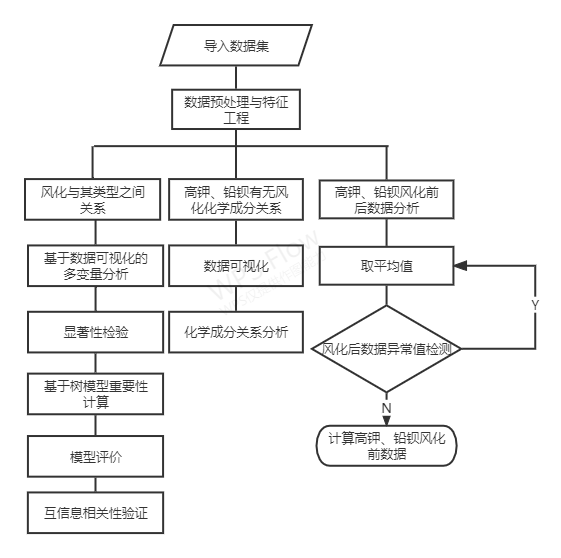
\includegraphics[width=0.95\textwidth]{1.png} 
    % 最终文档中希望显示的图注
	\caption{流程图} 
    % 用于文内引用的标签,这个东西没什么用,但最好就是你按照文中的顺序把图片依次命名为1、2...,然后这个标签就跟着命名走
	\label{Fig.main1} 
\end{figure}

\subsection{问题三的分析}

问题分析内容问题分析内容问题分析内容问题分析内容问题分析内容问题分析内容问题分析内容问题分析内容问题分析内容问题分析内容问题分析内容问题分析内容问题分析内容问题分析内容问题分析内容问题分析内容问题分析内容问题分析内容问题分析内容问题分析内容问题分析内容问题分析内容问题分析内容问题分析内容问题分析内容问题分析内容问题分析内容问题分析内容问题分析内容问题分析内容问题分析内容


\subsection{问题四的分析}

问题分析内容问题分析内容问题分析内容问题分析内容问题分析内容问题分析内容问题分析内容问题分析内容问题分析内容问题分析内容问题分析内容问题分析内容问题分析内容问题分析内容问题分析内容问题分析内容问题分析内容问题分析内容问题分析内容问题分析内容问题分析内容问题分析内容问题分析内容问题分析内容问题分析内容问题分析内容问题分析内容问题分析内容问题分析内容问题分析内容问题分析内容

